% Vilnius University beamer template
% Bakalauro baigiamojo darbo gynimas – Gvidas Bačianskas, 2026

\documentclass[12pt]{beamer}

\renewcommand{\figurename}{}
\renewcommand{\tablename}{}
\renewcommand\thefigure{\arabic{figure} pav.}
\renewcommand\thetable{\arabic{table} lentelė.}

\usepackage{graphicx}
\usepackage{caption}
\usepackage{subfig}
\usepackage{hyperref}

\usetheme{Madrid}

\title[]{TurtleBot Burger robotui skirtų aplinkos išžvalgymo algoritmų palyginimas realiose sąlygose}
\subtitle[]{Bakalauro baigiamasis darbas}
\author[Gvidas Bačianskas]{Gvidas Bačianskas}
\date{}

\addtobeamertemplate{author}{}{Darbo vadovas: prof. dr. Virginijus Marcinkevičius\par}
\addtobeamertemplate{author}{}{Darbo recenzentas: doc. dr. Valentas Gružauskas\par}

\setbeamertemplate{navigation symbols}{}
\titlegraphic{
\includegraphics[width=2cm]{resources/MIF.png}}

\usepackage{VUMIF}
\usepackage[T1]{fontenc}

\begin{document}

%% 1. Titulinis
\begin{frame}
    \titlepage
\end{frame}

%% 2. Įvadas
\begin{frame}{Įvadas}
    \textbf{Tyrimo problema:}
    \begin{itemize}
        \item Autonominiams robotams nepakanka sudaryti žemėlapio -- robotas turi nuspręsti, kurią neištirtą aplinkos dalį tirti toliau
        \item Skirtingais sprendimų priėmimo principais pagrįsti metodai gali nevienodai veikti skirtingos geometrijos realiose patalpose
        \item Nėra aišku, kuris metodas tinkamesnis paprastoje patalpoje, dviejų kambarių aplinkoje ar ilgame koridoriuje
    \end{itemize}

    \vspace{0.4cm}
    \textbf{Darbo tikslas:}
    \begin{itemize}
        \item Palyginti penkis aplinkos išžvalgymo algoritmus, įgyvendintus vienoje ROS~2 ir TurtleBot~Burger roboto architektūroje, taikant palyginamas realių vidaus patalpų eksperimentų sąlygas
    \end{itemize}
\end{frame}

%% 3. Darbo uždaviniai
\begin{frame}{Darbo uždaviniai}
    \begin{enumerate}
        \item Įvertinti pasirinktų aplinkos išžvalgymo algoritmų grupių teorinius principus ir nustatyti, kodėl jos tinkamos palyginti TurtleBot~Burger robotui realiomis sąlygomis
        \item Įgyvendinti penkis algoritmus vienoje ROS~2 programinėje architektūroje -- su bendru užimtumo tinklu, navigacija ir metrikų registravimu
        \item Apibrėžti palyginimo kriterijus ir eksperimentų eigą: padengimas, laikas, kelias, tikslų vykdymo rezultatai
        \item Surinkti palyginamus eksperimentinius duomenis trijose realiose vidaus aplinkose
        \item Palyginti algoritmų rezultatus pagal nustatytas metrikas kiekvienoje aplinkoje
        \item Suformuluoti praktines rekomendacijas, kuris algoritmas tinkamesnis skirtingoms aplinkų geometrijoms
    \end{enumerate}
\end{frame}

%% 4. Literatūros analizė – algoritmų grupės
\begin{frame}{Aplinkos išžvalgymo algoritmų grupės}
    \begin{columns}[onlytextwidth]
        \column{0.52\textwidth}
        \textbf{Penki lyginami algoritmai:}
        \begin{enumerate}
            \item \textbf{BFS} -- grafų paieška per žinomą laisvą erdvę
            \item \textbf{Artimiausios ribos} -- klasikinis ribomis pagrįstas metodas
            \item \textbf{RRT} -- atsitiktinė imtis ir medžio augimas
            \item \textbf{Informacijos prieaugis} -- naudingumo funkcija pagrįstas vertinimas
            \item \textbf{Voronoi} -- laisvos erdvės geometrinė ir topologinė struktūra
        \end{enumerate}

        \column{0.48\textwidth}
        \textbf{Bendra palyginimo sąlyga:}
        \begin{itemize}
            \item Visi algoritmai gauna tą patį \textbf{užimtumo tinklą} ir roboto poziciją
            \item Visi siunčia tikslus per tą pačią \textbf{Nav2} sąsają
            \item Skirtumai -- tik \textbf{tikslo parinkimo strategijoje}
        \end{itemize}

        \vspace{0.3cm}
        $\Rightarrow$ Lyginami \textbf{sprendimų priėmimo principai}, ne sistemos skirtumai
    \end{columns}
\end{frame}

%% 5. TurtleBot3 Burger platforma
\begin{frame}{TurtleBot3 Burger platforma}
    \begin{columns}[onlytextwidth]
        \column{0.56\textwidth}
        \textbf{Pagrindiniai komponentai:}
        \begin{itemize}
            \item \textbf{Dynamixel XM430} -- varikliai su integruotais enkoderiais
            \item \textbf{OpenCR} -- žemo lygio mikrovaldiklis: variklių valdymas, odometrija
            \item \textbf{Raspberry Pi 3} -- pagrindinis kompiuteris: ROS~2, SLAM, navigacija
            \item \textbf{LiDAR LDS-02} -- 360° lazerinis jutiklis (0,16--8~m)
        \end{itemize}

        \vspace{0.2cm}
        \textbf{Aplinkos modelis:}
        \begin{itemize}
            \item Užimtumo tinklas (0,05~m/langelis)
            \item SLAM Toolbox -- grafų optimizavimo SLAM
        \end{itemize}
        \column{0.44\textwidth}
        \begin{figure}
            \centering
            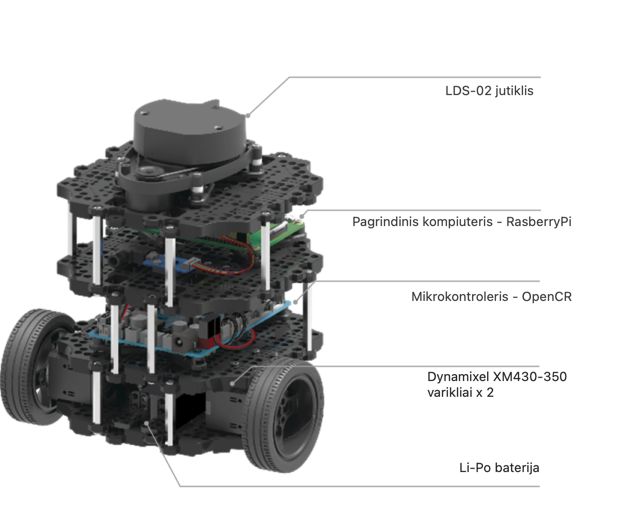
\includegraphics[width=0.88\textwidth]{../BBD-dokumentas/BakBaigDarb/images/TurtleBot.png}
            \caption{TurtleBot3 Burger}
        \end{figure}
    \end{columns}
\end{frame}

%% 6. Sistemos architektūra
\begin{frame}{Sistemos architektūra}
    \begin{columns}[onlytextwidth]
        \column{0.46\textwidth}
        \textbf{Komponentai:}
        \begin{itemize}
            \item \textbf{Fiziniai:} TurtleBot Burger + LDS-02
            \item \textbf{SLAM:} slam\_toolbox -- žemėlapio sudarymas
            \item \textbf{Navigacija:} Nav2 -- kelių planavimas ir vykdymas
            \item \textbf{Išžvalgymas:} main\_node.py -- pagrindinis ciklas; \textit{Strategija} -- vienas iš 5 algoritmų
        \end{itemize}

        \vspace{0.2cm}
        Strategija parenkama \textbf{paleidimo metu} -- visi kiti komponentai nesikeičia
        \column{0.54\textwidth}
        \begin{figure}
            \centering
            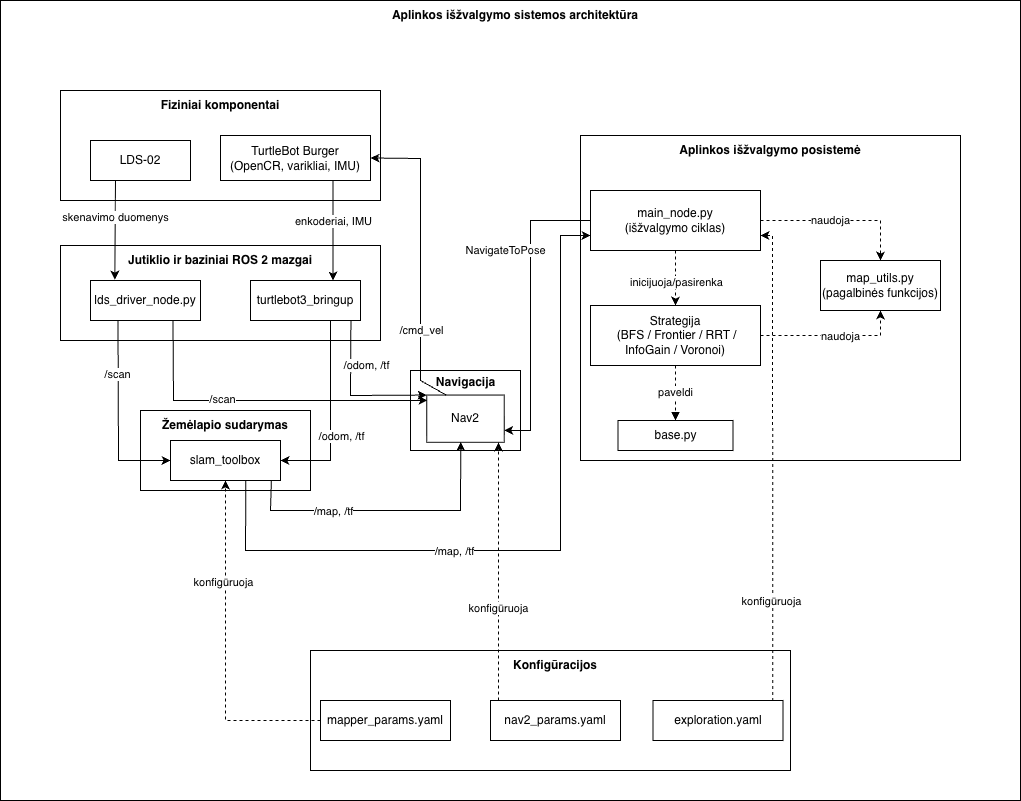
\includegraphics[width=\textwidth]{../BBD-dokumentas/BakBaigDarb/images/diagramos/sysarch.png}
            \caption{Aplinkos išžvalgymo sistemos architektūra}
        \end{figure}
    \end{columns}
\end{frame}

%% 7. BFS ir Artimiausios ribos
\begin{frame}{BFS ir Artimiausios ribos algoritmai}
    \begin{columns}[onlytextwidth]
        \column{0.5\textwidth}
        \textbf{BFS algoritmas}
        \begin{itemize}
            \item Pločio paieška per laisvą užimtumo tinklo sritį pradedant nuo roboto
            \item Randa \textbf{pirmą pasiekiamą} ribinį langelį
            \item Tikslas perkeliamas atgal į žinomą erdvę (\textit{goal\_standoff})
            \item[+] Sistemingai aptinka pasiekiamas ribas
            \item[--] Smulkūs, arti esantys tikslai; daug navigacijos žingsnių
        \end{itemize}

        \column{0.5\textwidth}
        \textbf{Artimiausios ribos algoritmas}
        \begin{itemize}
            \item Aptinkamos \textbf{visos} ribinės sritys užimtumo tinkle
            \item Kiekvienai apskaičiuojamas reprezentacinis centroido taškas
            \item Pasirenkama \textbf{arčiausiai roboto} esanti riba (Euklido atstumas)
            \item[+] Paprastas, deterministinis, stabilus
            \item[--] Gali nepasirinkti informatyviausios ribos
        \end{itemize}
    \end{columns}
\end{frame}

%% 8. RRT, Informacijos prieaugis, Voronoi
\begin{frame}{RRT, Informacijos prieaugis ir Voronoi algoritmai}
    \small
    \textbf{RRT} -- atsitiktinis medžio augimas (\textit{Rapidly-exploring Random Tree})
    \begin{itemize}
        \item Atsitiktinai imami taškai žemėlapio ribose; medis plečiamas link jų
        \item Ribiniai lapai -- kandidatai; vertinami pagal $S = I - w \cdot C$
        \item[--] Stochastinis -- rezultatai gali labai skirtis tarp bandymų
    \end{itemize}

    \vspace{0.2cm}
    \textbf{Informacijos prieaugis} -- naudingumo funkcija pagrįstas ribų vertinimas
    \begin{itemize}
        \item Visos ribos vertinamos pagal tikėtiną atskleidžiamą nežinomų langelių skaičių
        \item $S = \alpha \cdot I_n + (1-\alpha) \cdot C_n$ \quad ($\alpha = 0{,}7$) -- derina informatyvumą su artumu
    \end{itemize}

    \vspace{0.2cm}
    \textbf{Voronoi} -- laisvos erdvės geometrinė struktūra (GVD)
    \begin{itemize}
        \item Atstumo transformacija $\rightarrow$ keterų skeletas $\rightarrow$ grafas
        \item Ribos vertinamos pagal $U_f = I_f - h \cdot N_f$; perduodama tarpinių taškų seka
        \item[+] Kelias palei saugesnes laisvos erdvės vietas
        \item[--] Ilgesnis kelias; sudėtingesnė realizacija
    \end{itemize}
\end{frame}

%% 9. Eksperimentinės aplinkos
\begin{frame}{Eksperimentinės aplinkos}
    \begin{columns}[onlytextwidth]
        \column{0.33\textwidth}
        \centering
        \textbf{1 aplinka}\\
        \small\textit{Kambarys su objektais}\\
        \vspace{0.15cm}
        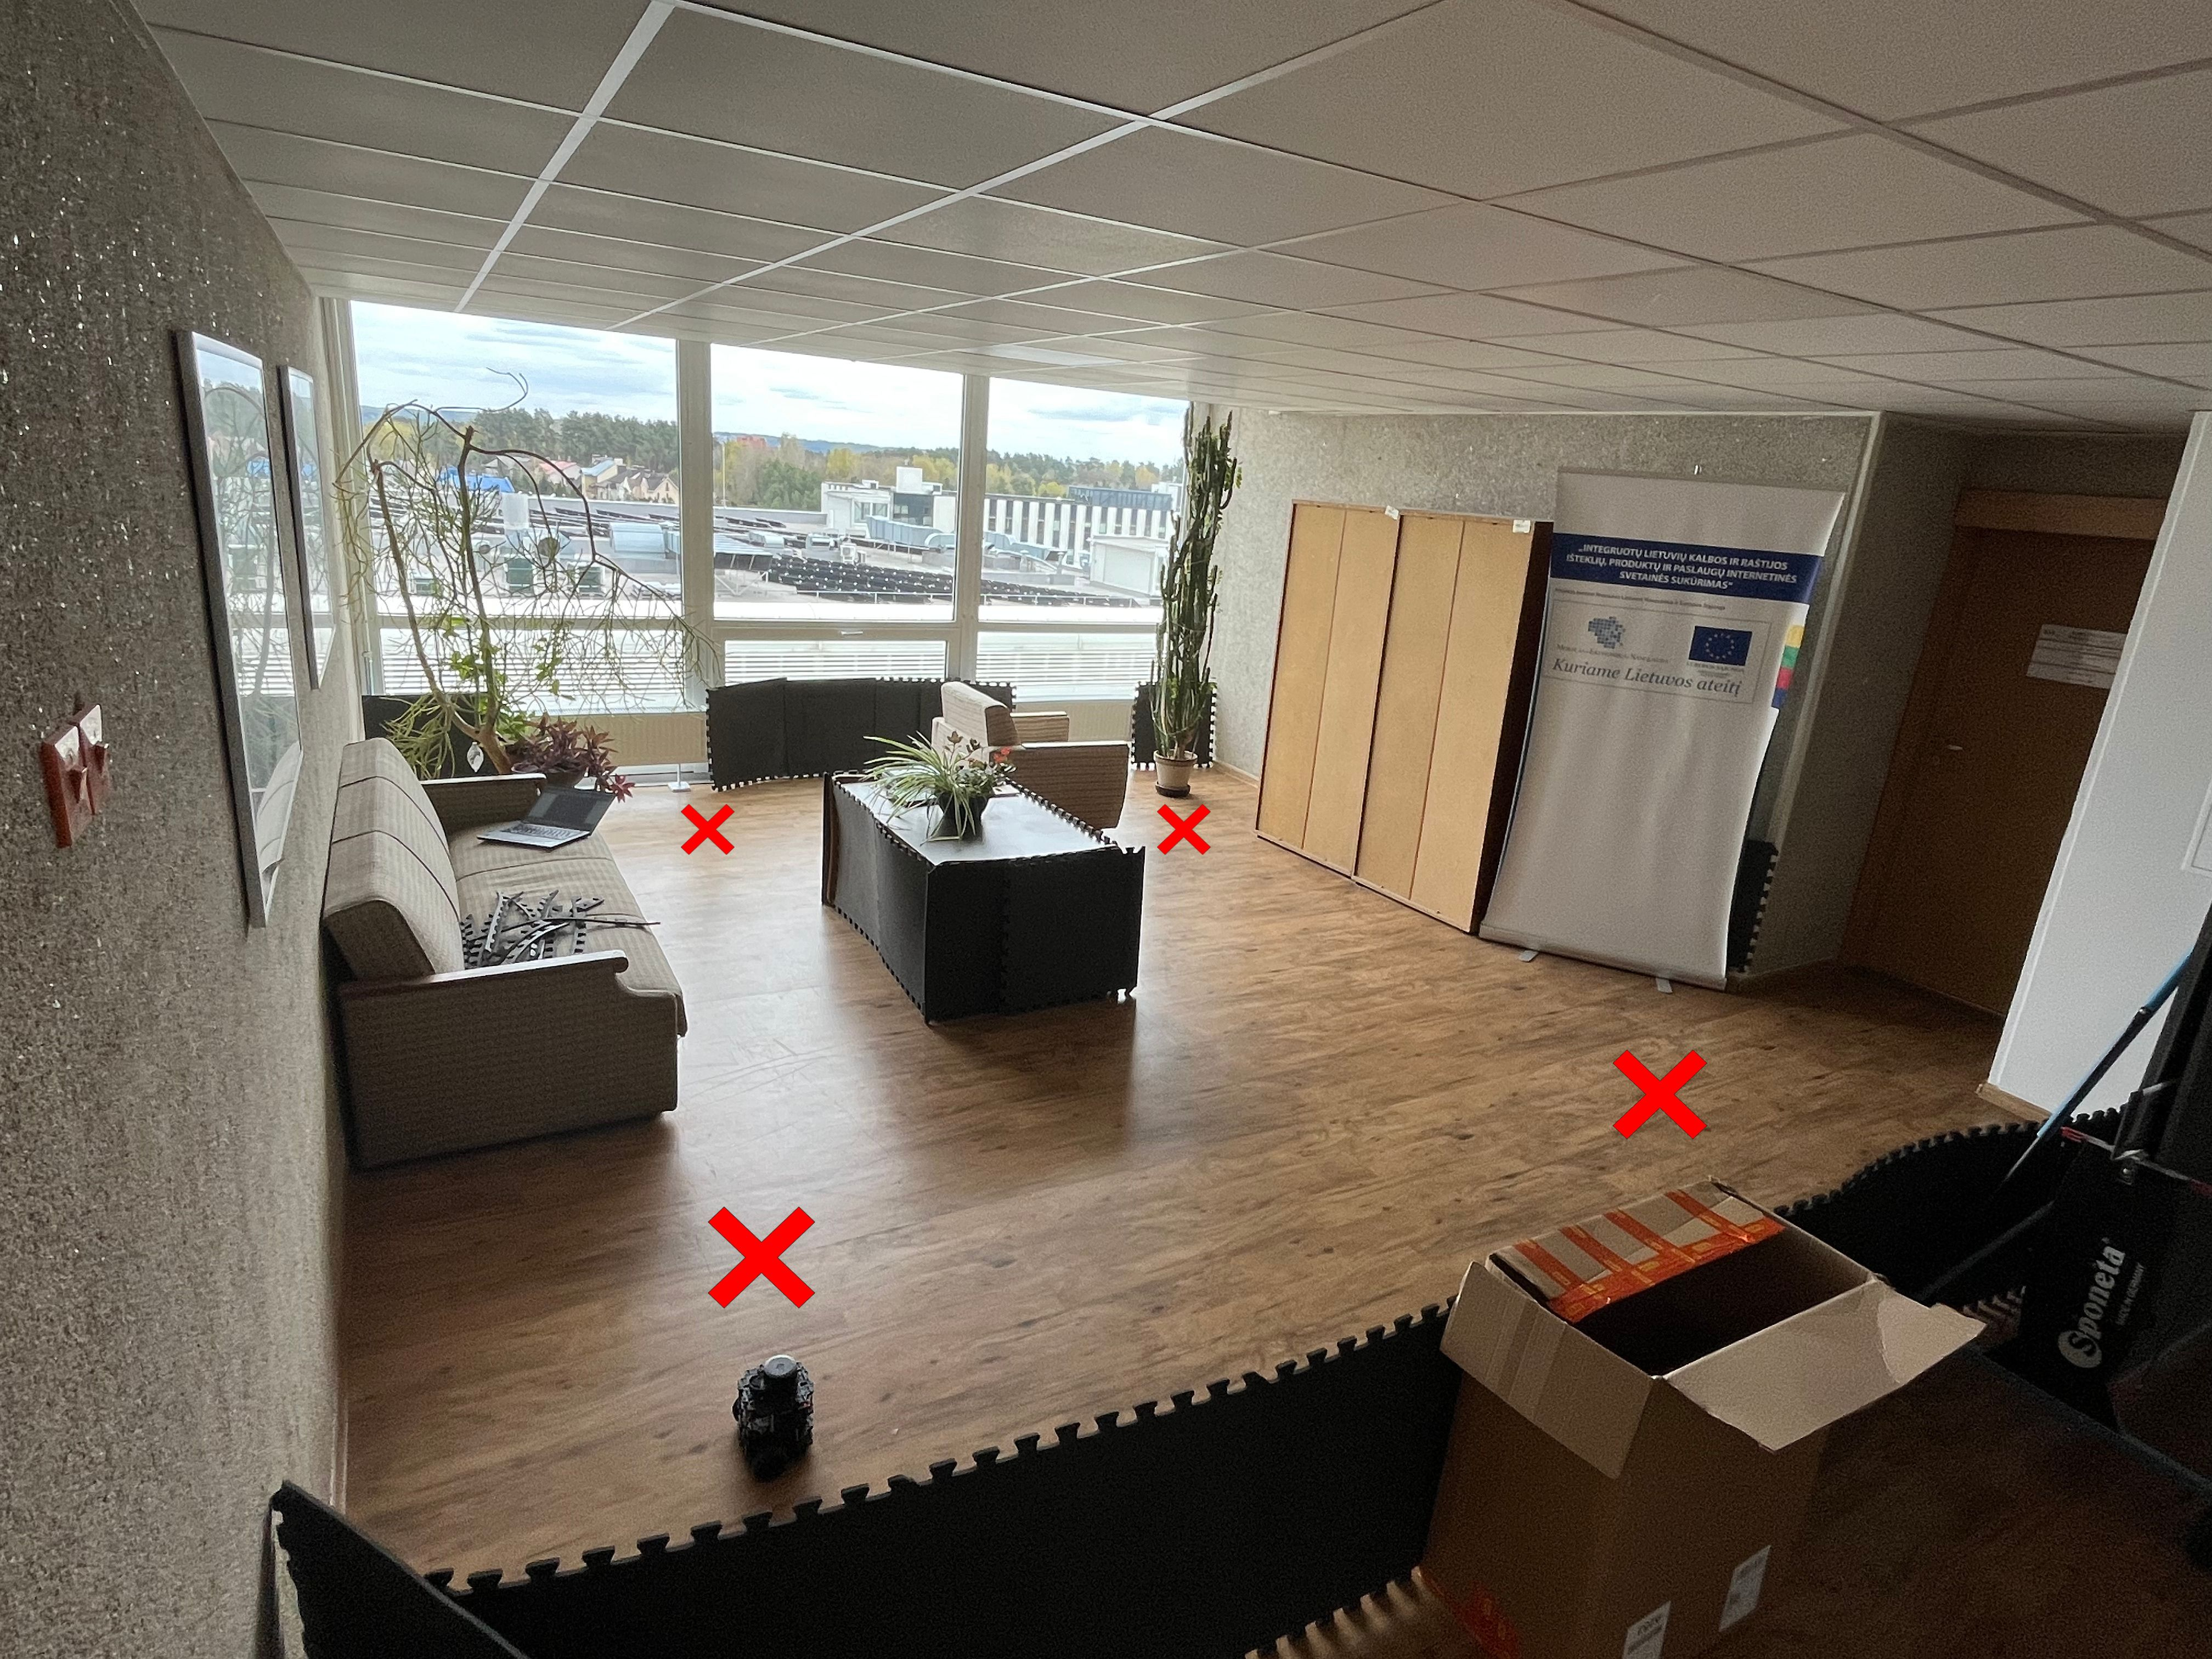
\includegraphics[width=\textwidth]{../BBD-dokumentas/BakBaigDarb/images/kamb1/1-w-marks.jpg}\\
        \vspace{0.1cm}
        \footnotesize $\approx7 \times 6{,}5$~m\\4 bandymai

        \column{0.33\textwidth}
        \centering
        \textbf{2 aplinka}\\
        \small\textit{Du kambariai + siauras praėjimas}\\
        \vspace{0.15cm}
        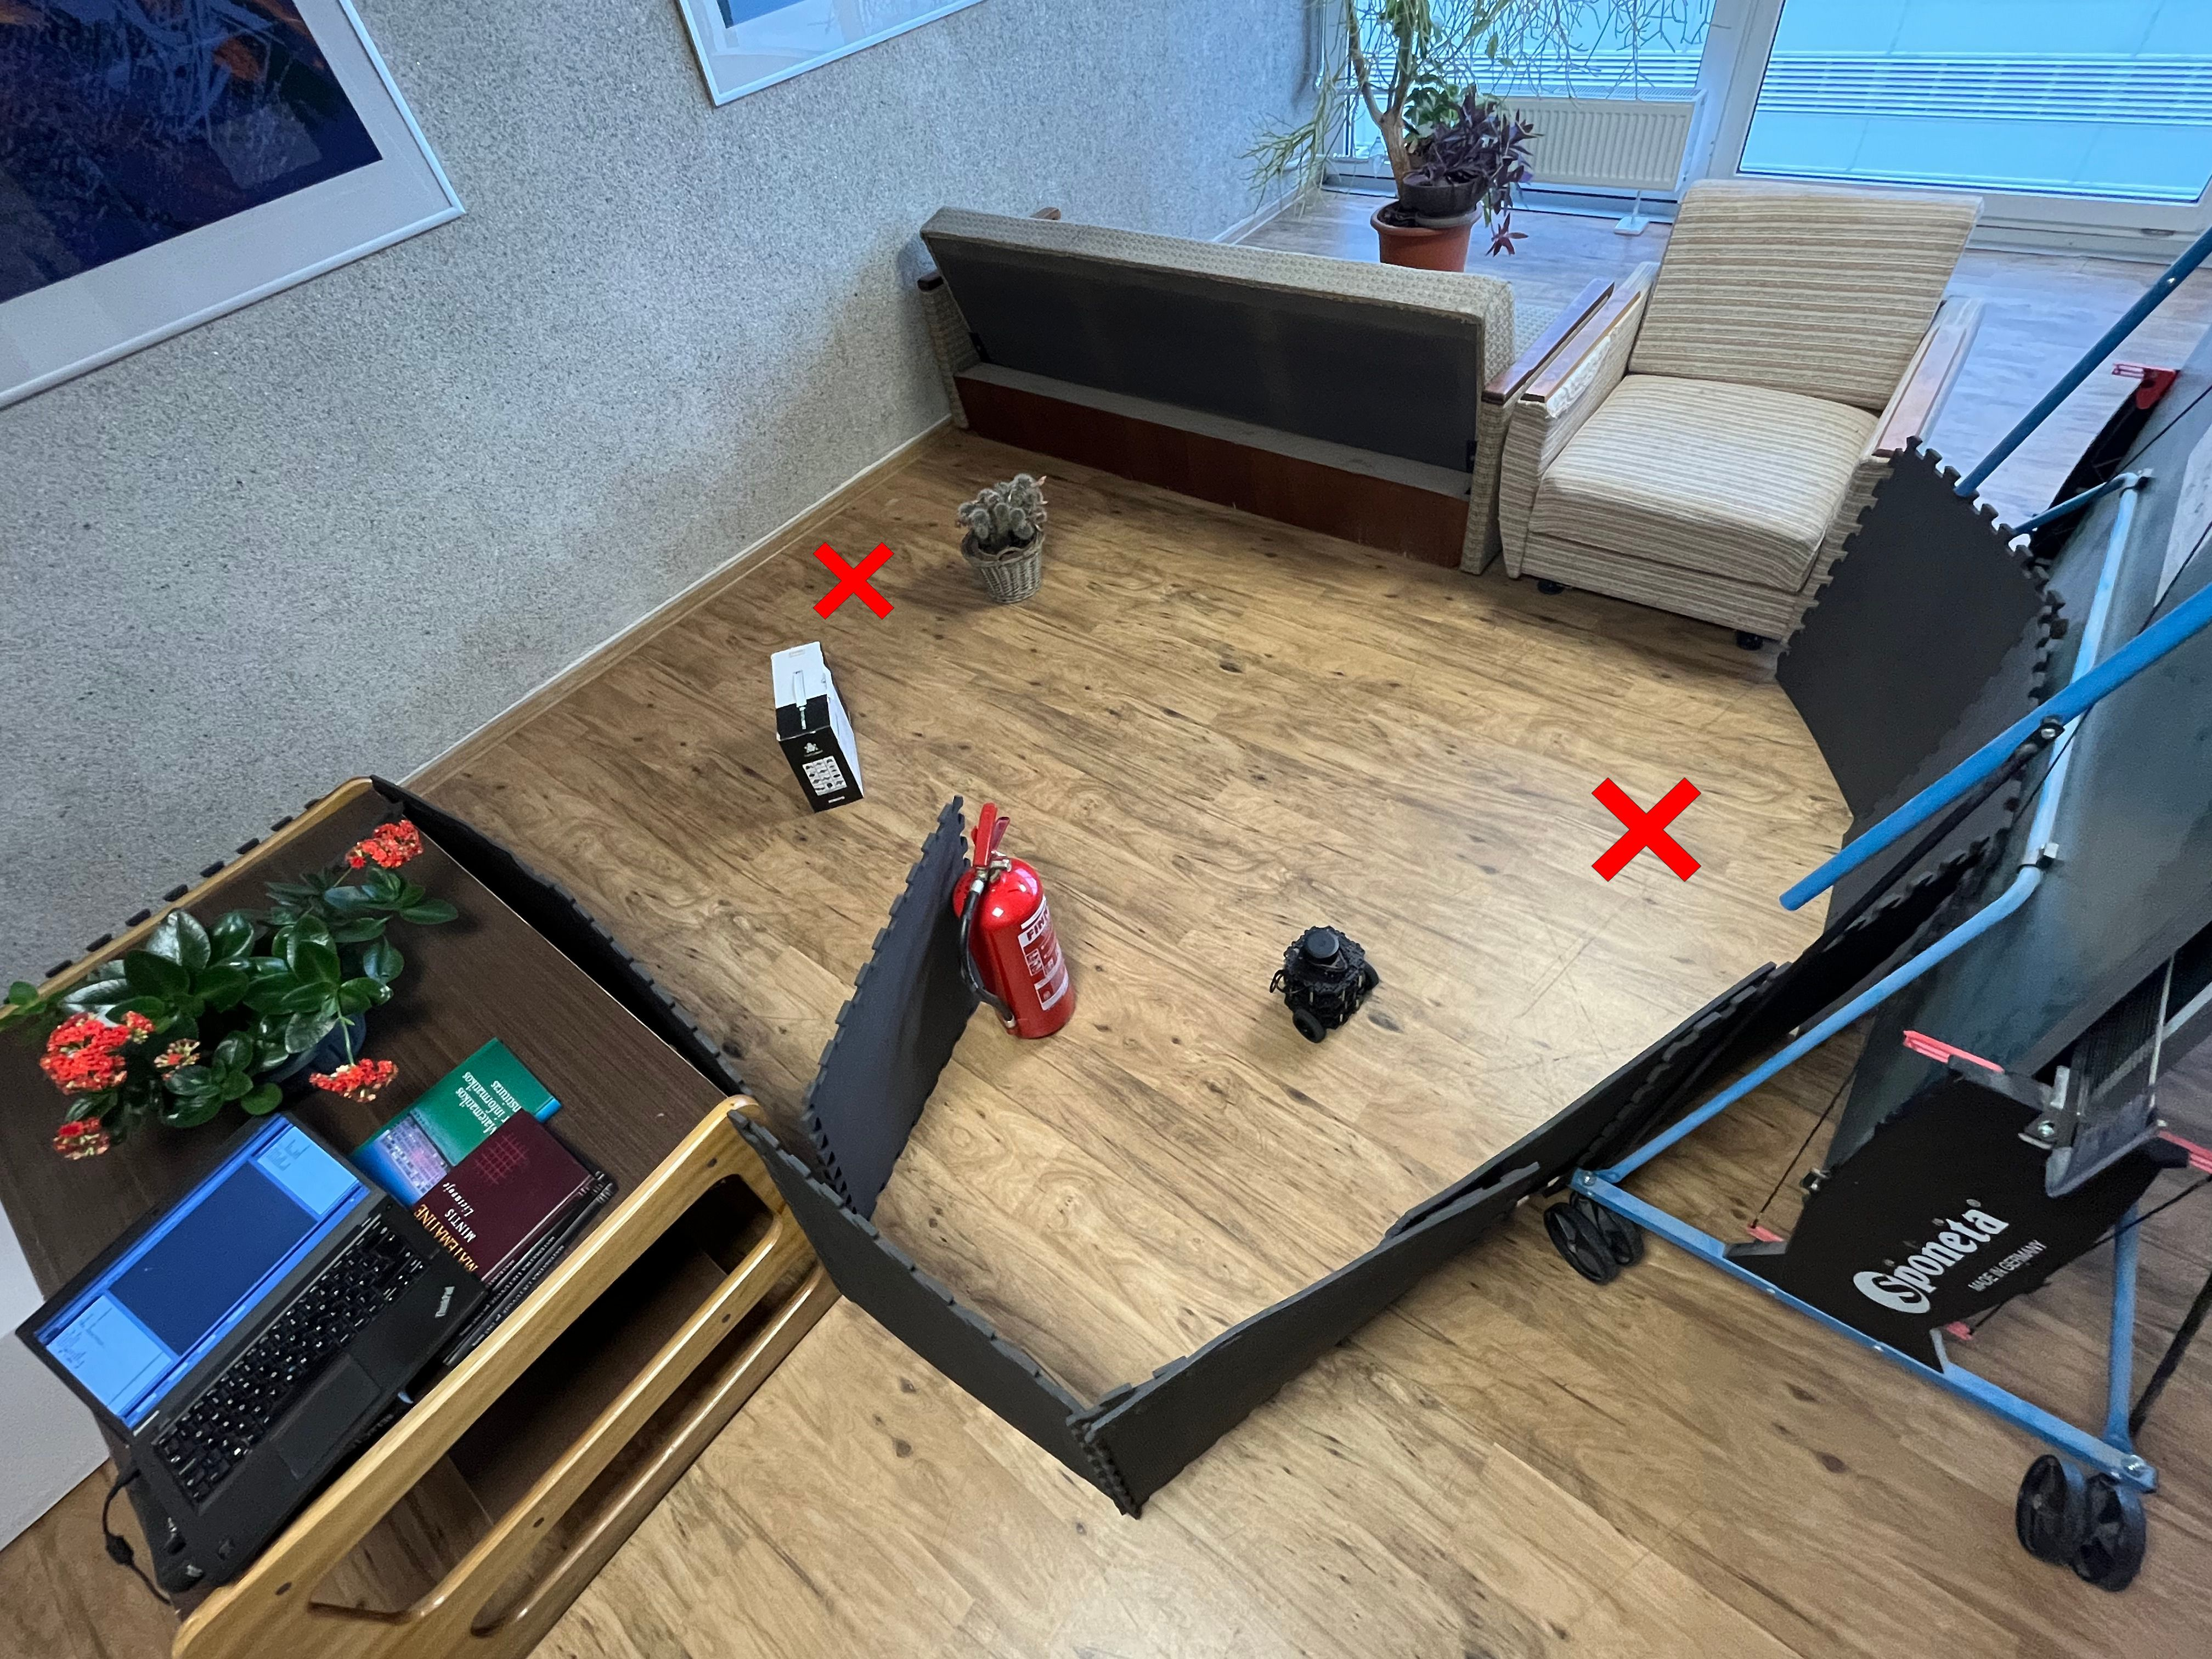
\includegraphics[width=\textwidth]{../BBD-dokumentas/BakBaigDarb/images/kamb2/1-w-marks.jpg}\\
        \vspace{0.1cm}
        \footnotesize $3{,}5{\times}3{,}5$ + $3{\times}2{,}5$~m\\4 bandymai

        \column{0.33\textwidth}
        \centering
        \textbf{3 aplinka}\\
        \small\textit{Ilgas koridorius + nišos}\\
        \vspace{0.15cm}
        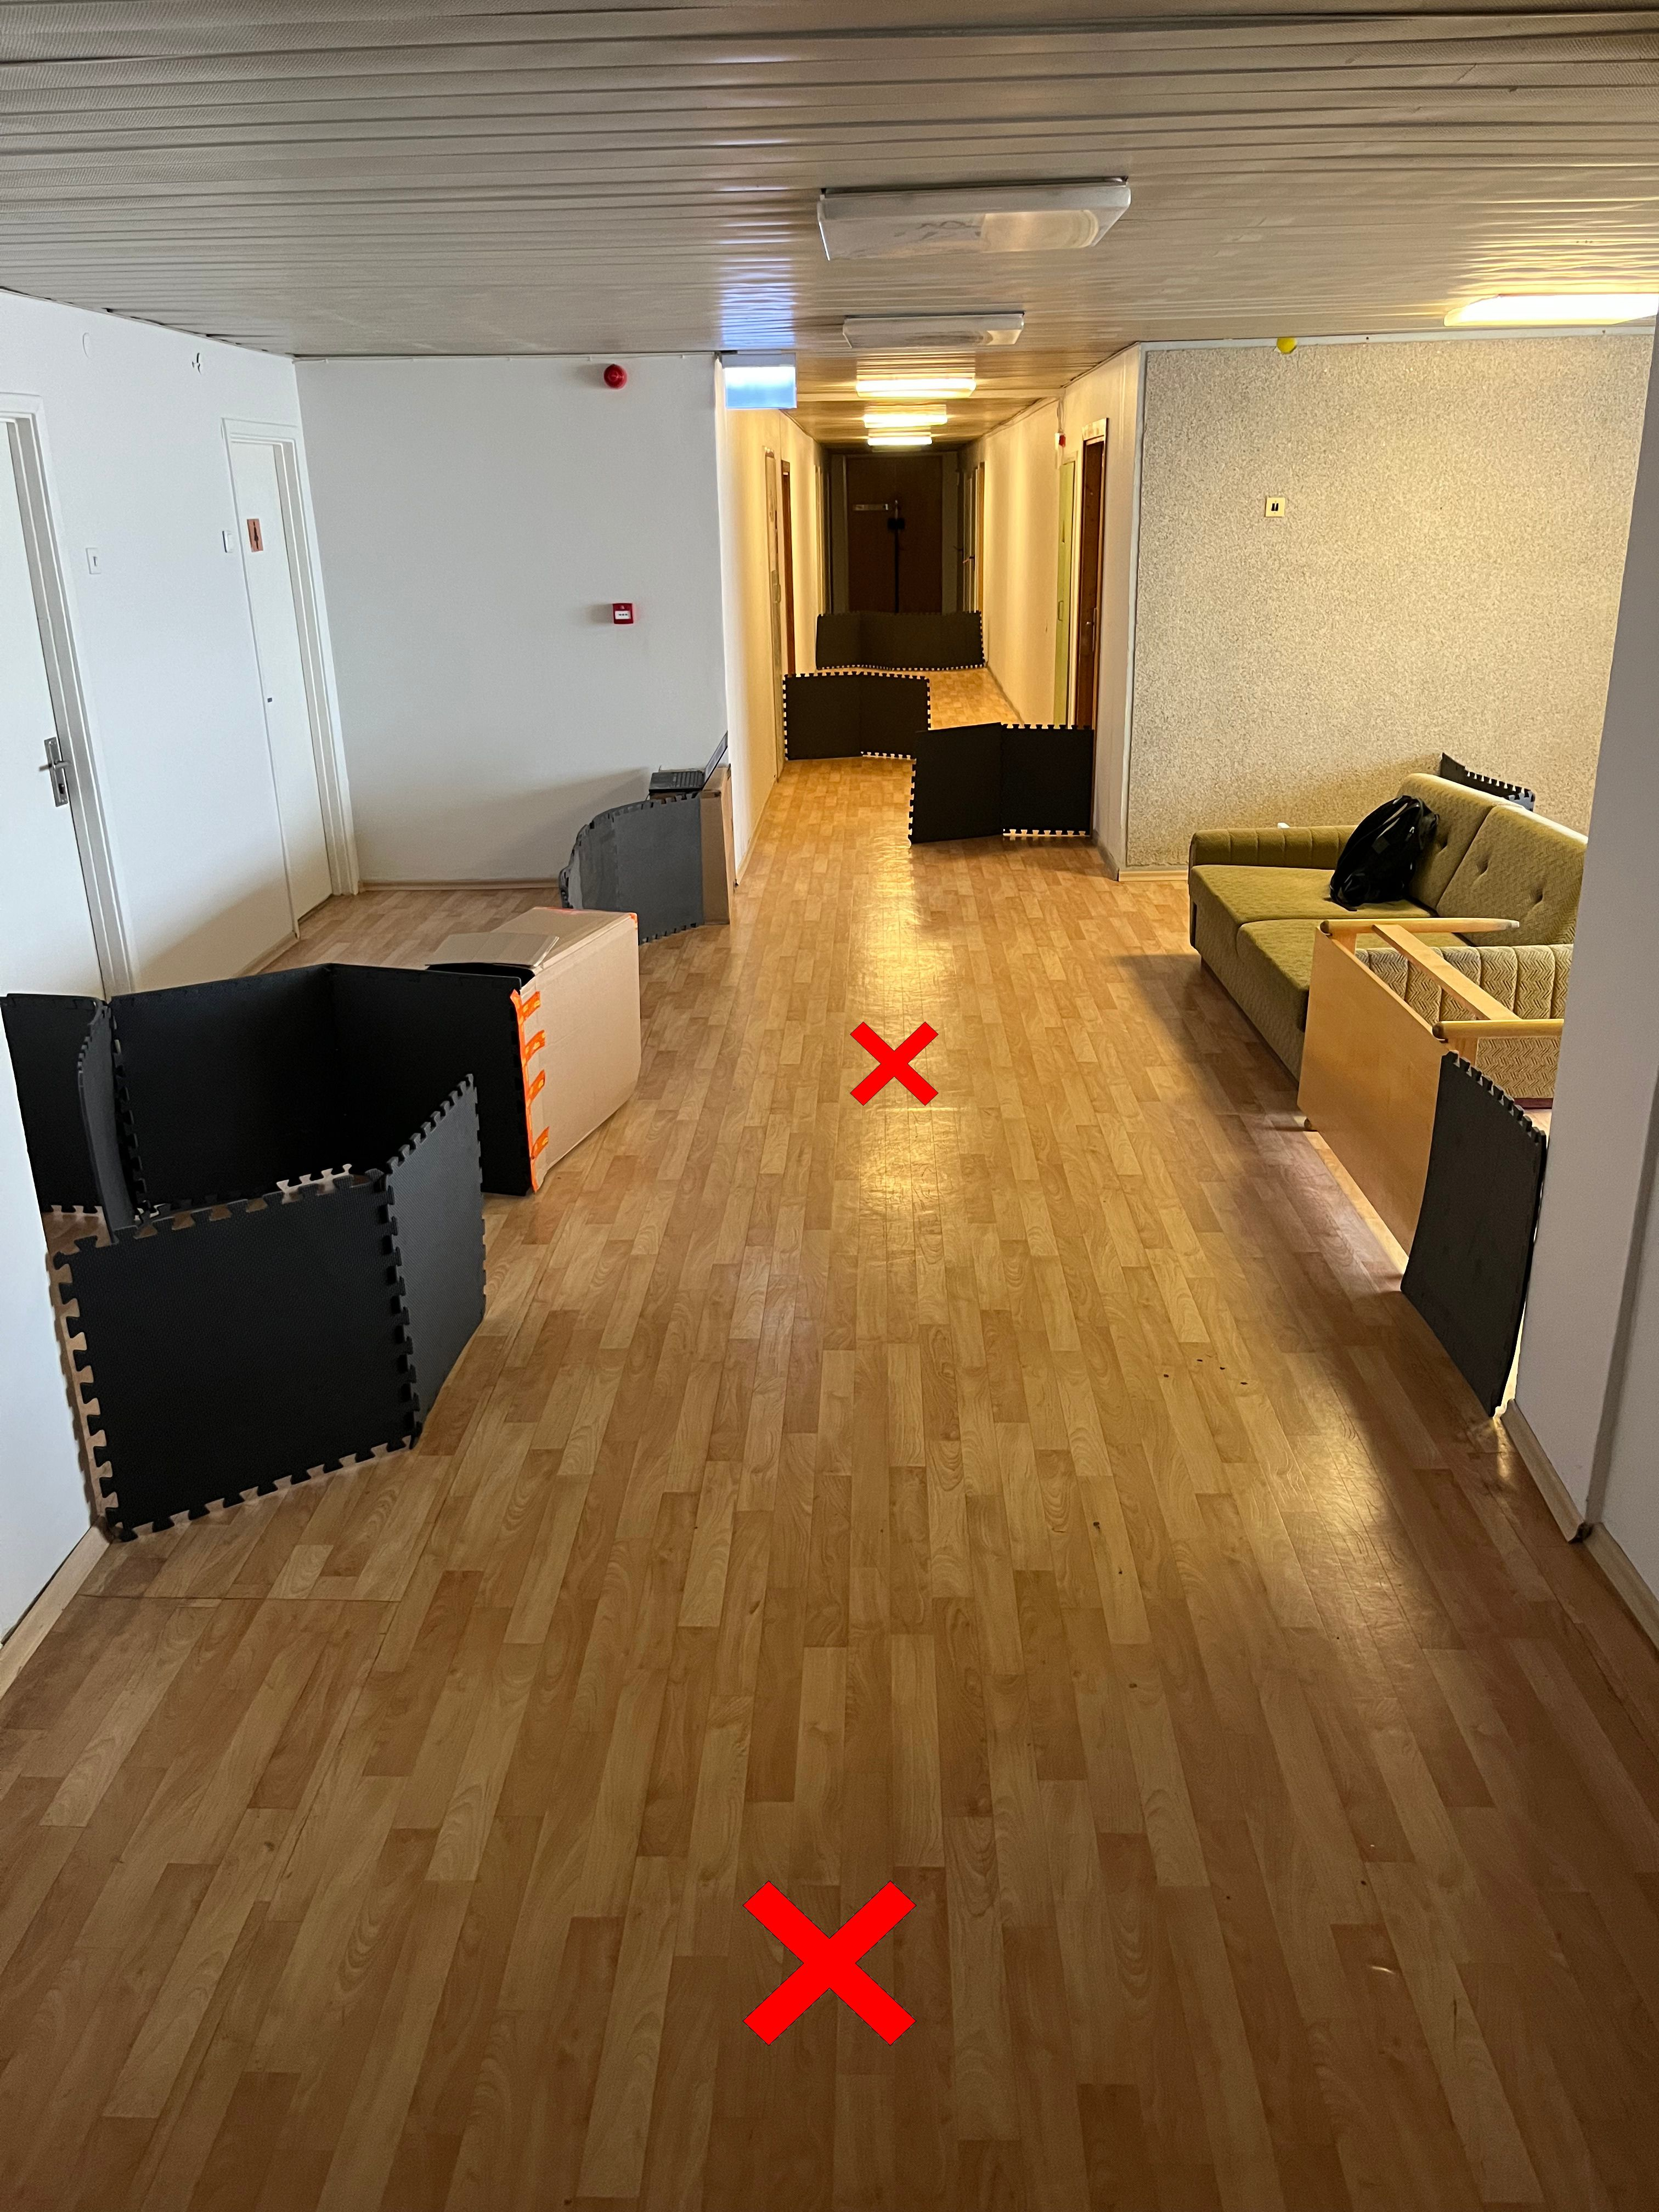
\includegraphics[width=\textwidth]{../BBD-dokumentas/BakBaigDarb/images/kamb3/2-w-marks.jpg}\\
        \vspace{0.1cm}
        \footnotesize $24 \times 2{,}5$~m\\3 bandymai
    \end{columns}
\end{frame}

%% 10. Eksperimentų metodika
\begin{frame}{Eksperimentų metodika}
    \begin{columns}[onlytextwidth]
        \column{0.55\textwidth}
        \textbf{Palyginimo metrikos:}
        \begin{itemize}
            \item Išžvalgymo trukmė (s)
            \item Žemėlapio padengimas (\%)
            \item Roboto nuvažiuotas kelias (m)
            \item Išsiųstų / pasiektų / \textbf{nepavykusių} navigacijos tikslų skaičius
        \end{itemize}

        \vspace{0.3cm}
        \textbf{Palyginamumo užtikrinimas:}
        \begin{itemize}
            \item Tos pačios pradinės pozicijos visiems algoritmams
            \item Ta pati Nav2 ir SLAM Toolbox konfigūracija
            \item Keičiasi tik \textbf{išžvalgymo strategija}
        \end{itemize}

        \column{0.45\textwidth}
        \textbf{Eksperimento pabaigos sąlyga:}
        \begin{itemize}
            \item 8 ciklai iš eilės be naujo tikslo
            \item \textit{goal\_timeout} = 60~s
            \item \textit{failure\_cooldown} = 3~s
        \end{itemize}

        \vspace{0.3cm}
        \textbf{Rezultatų pateikimas:}
        \begin{itemize}
            \item Bandymų vidurkiai
            \item Rezultatų intervalai
            \item Standartinis nuokrypis (stabilumo vertinimui)
        \end{itemize}
    \end{columns}
\end{frame}

%% 11. Pirmosios aplinkos rezultatai
\begin{frame}{Pirmosios aplinkos rezultatai}
    \begin{columns}[onlytextwidth]
        \column{0.60\textwidth}
        \begin{table}
            \centering
            \footnotesize
            \begin{tabular}{|l|c|c|c|c|}
                \hline
                \textbf{Algoritmas} & \textbf{Laikas, s} & \textbf{Padeng., \%} & \textbf{Kelias, m} & \textbf{Nepavyko} \\
                \hline
                BFS & 244,4 & \textbf{96,6} & 17,26 & 1,0 \\
                \hline
                Art. riba & 207,9 & 95,2 & \textbf{14,77} & 1,0 \\
                \hline
                Info prieaugis & 242,2 & 95,3 & 18,01 & 2,5 \\
                \hline
                RRT & 202,2 & 95,0 & 16,43 & 0,8 \\
                \hline
                Voronoi & \textbf{200,9} & 95,2 & 17,40 & \textbf{0,5} \\
                \hline
            \end{tabular}
        \end{table}
        \vspace{0.2cm}
        \footnotesize
        Visi algoritmai pasiekė $\approx$95--97\% padengimą.\\
        Skirtumai nedideli -- paprasta, atvira aplinka.\\
        Voronoi -- greičiausias; Art. riba -- trumpiausias kelias.

        \column{0.40\textwidth}
        \begin{figure}
            \centering
            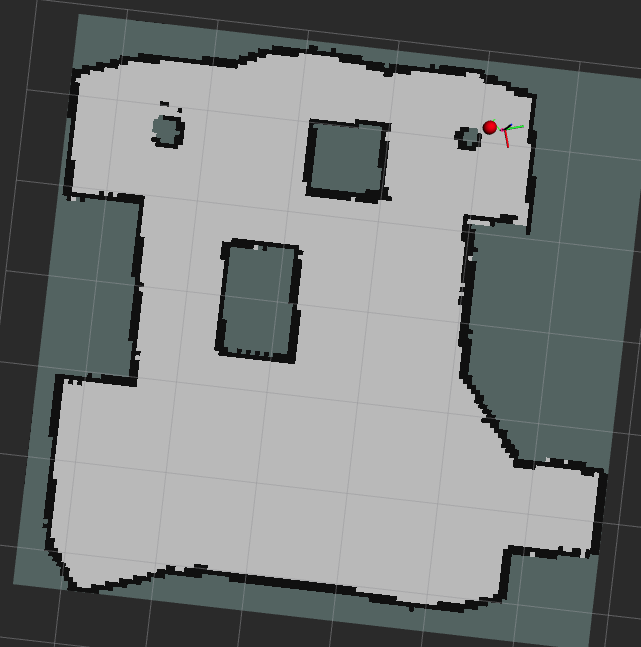
\includegraphics[width=\textwidth]{../BBD-dokumentas/BakBaigDarb/images/sudarytas_zemelap/1_kamb.png}
            \caption{Sudarytas žemėlapis}
        \end{figure}
    \end{columns}
\end{frame}

%% 12. Antrosios aplinkos rezultatai
\begin{frame}{Antrosios aplinkos rezultatai}
    \begin{columns}[onlytextwidth]
        \column{0.60\textwidth}
        \begin{table}
            \centering
            \footnotesize
            \begin{tabular}{|l|c|c|c|c|}
                \hline
                \textbf{Algoritmas} & \textbf{Laikas, s} & \textbf{Padeng., \%} & \textbf{Kelias, m} & \textbf{Nepavyko} \\
                \hline
                BFS & 358,7 & 98,4 & 20,02 & 3,0 \\
                \hline
                Art. riba & \textbf{162,1} & 98,4 & 13,79 & \textbf{0,0} \\
                \hline
                Info prieaugis & 172,8 & 98,4 & \textbf{13,56} & \textbf{0,0} \\
                \hline
                RRT & 203,4 & 98,3 & 17,62 & 1,0 \\
                \hline
                Voronoi & 224,7 & \textbf{98,5} & 18,67 & 1,0 \\
                \hline
            \end{tabular}
        \end{table}
        \vspace{0.2cm}
        \footnotesize
        Artimiausios ribos ir informacijos prieaugis -- \textbf{0 nesėkmingų tikslų}.\\
        BFS -- ilgiausias laikas (358,7~s) ir daugiausiai nesėkmių (3,0).\\
        Siauras praėjimas išryškino metodų skirtumus.

        \column{0.40\textwidth}
        \begin{figure}
            \centering
            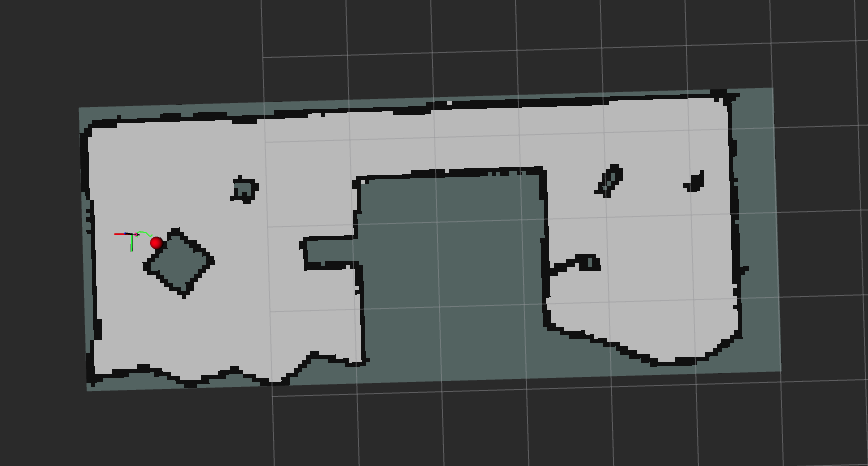
\includegraphics[width=\textwidth]{../BBD-dokumentas/BakBaigDarb/images/sudarytas_zemelap/2_kamb.png}
            \caption{Sudarytas žemėlapis}
        \end{figure}
    \end{columns}
\end{frame}

%% 13. Trečiosios aplinkos rezultatai
\begin{frame}{Trečiosios aplinkos rezultatai}
    \begin{columns}[onlytextwidth]
        \column{0.60\textwidth}
        \begin{table}
            \centering
            \footnotesize
            \begin{tabular}{|l|c|c|c|c|}
                \hline
                \textbf{Algoritmas} & \textbf{Laikas, s} & \textbf{Padeng., \%} & \textbf{Kelias, m} & \textbf{Nepavyko} \\
                \hline
                BFS & 533,6 & \textbf{100,0} & 37,74 & 1,7 \\
                \hline
                Art. riba & 342,9 & 99,9 & 31,69 & 3,0 \\
                \hline
                Info prieaugis & \textbf{259,1} & \textbf{100,0} & \textbf{27,28} & \textbf{0,3} \\
                \hline
                RRT & 418,7 & 99,7 & 38,42 & 4,0 \\
                \hline
                Voronoi & 567,9 & \textbf{100,0} & 54,50 & 5,7 \\
                \hline
            \end{tabular}
        \end{table}
        \vspace{0.2cm}
        \footnotesize
        Informacijos prieaugis -- \textbf{geriausias pagal visas metrikas}.\\
        Voronoi -- ilgiausias kelias (54,50~m) ir daugiausiai nesėkmių (5,7).\\
        Koridoriuje tolimaregiškas tikslo pasirinkimas pasiteisino.

        \column{0.40\textwidth}
        \begin{figure}
            \centering
            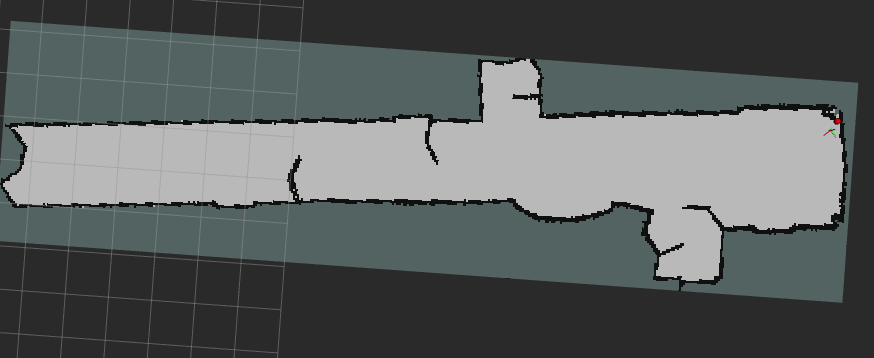
\includegraphics[width=\textwidth]{../BBD-dokumentas/BakBaigDarb/images/sudarytas_zemelap/3_kamb.png}
            \caption{Sudarytas žemėlapis}
        \end{figure}
    \end{columns}
\end{frame}

%% 14. Rezultatų suvestinė
\begin{frame}{Rezultatų suvestinė}
    \textbf{Bendras rangavimas} (5--1 taškai už kiekvieną metriką kiekvienoje aplinkoje):

    \begin{table}
        \centering
        \small
        \begin{tabular}{|l|c|c|c|c|c|}
            \hline
            \textbf{Algoritmas} & \textbf{1 aplinka} & \textbf{2 aplinka} & \textbf{3 aplinka} & \textbf{Iš viso} & \textbf{Vieta} \\
            \hline
            BFS & 9 & 6 & 10 & 25 & 5 \\
            \hline
            \textbf{Artimiausios ribos} & \textbf{11} & \textbf{13} & \textbf{12} & \textbf{36} & \textbf{1} \\
            \hline
            Informacijos prieaugis & 7 & 13 & 15 & 35 & 2 \\
            \hline
            RRT & 10 & 9 & 8 & 27 & 3 \\
            \hline
            Voronoi & 10 & 9 & 7 & 26 & 4 \\
            \hline
        \end{tabular}
    \end{table}

    \vspace{0.2cm}
    \begin{columns}[onlytextwidth]
        \column{0.5\textwidth}
        \textbf{Geriausias pagal aplinką:}
        \begin{itemize}
            \item 1 aplinka: Voronoi (laikas), Art. riba (kelias)
            \item 2 aplinka: Art. riba (laikas, 0 nesėkmių)
            \item 3 aplinka: Info prieaugis (visos metrikos)
        \end{itemize}
        \column{0.5\textwidth}
        \textbf{Rekomendacija:}
        \begin{itemize}
            \item Paprastos ir vidutinės aplinkos:\\
                  \textbf{artimiausios ribos} arba \textbf{informacijos prieaugis}
            \item Koridoriaus tipo aplinkos:\\
                  \textbf{informacijos prieaugis}
        \end{itemize}
    \end{columns}
\end{frame}

%% 15. Išvados
\begin{frame}{Išvados}
    \begin{enumerate}
        \item Visi penki algoritmai sėkmingai išžvalgė realias vidaus patalpas; veikimas priklausė nuo aplinkos geometrijos
        \item \textbf{BFS} dažnai pasiekė aukštą padengimą, tačiau generavo daugiausiai tikslų ir buvo lėčiausias
        \item \textbf{Artimiausios ribos} pasižymėjo stabilumu visose aplinkose -- \textbf{1 vieta} bendrai (36 taškai)
        \item \textbf{Informacijos prieaugis} buvo efektyviausias koridoriuje ir antras bendrai (35 taškai) -- geras balansas tarp laiko, kelio ir padengimo
        \item \textbf{RRT} ir \textbf{Voronoi} pasiekė aukštą padengimą, tačiau jų rezultatų kintamumas buvo didesnis
        \item Galutinis žemėlapio padengimas nėra pakankama metrika -- būtina vertinti ir laiką, kelią bei navigacijos nesėkmes
        \item Nėra universaliai geriausio algoritmo -- pasirinkimas turi būti siejamas su \textbf{aplinkos geometrija ir priimtinu kompromisu}
    \end{enumerate}
\end{frame}

%% 16. Ačiū
\begin{frame}
    \begin{center}
        \Huge Ačiū už dėmesį
    \end{center}
\end{frame}

\end{document}
